\chapter[Considerações sobre os Elementos Textuais]{Introdução}

\section{Contexto}

A tecnologia tem vindo a evoluir rapidamente e, com isto, nota-se o surgimento de
diversos desafios. Um destes desafios é a falta de programadores que possuam competências 
e qualificação necessárias para solucionar os mais diversos problemas presentes nos mais
variados projetos. Este fato está relacionado com a metodologia adotada no ensino de
programação e também com a falta de motivação por parte dos estudantes. \cite{7975788}.

\cite{inproceedings} afirma que uma das razões de os alunos não absorverem eficientemente
os conceitos relacionados à programação se dá pela falta de concentração dos mesmos frente
a exposição destes conteúdos na forma tradicional.

\cite{funcional} destaca que a aprendizagem dos conceitos e mecanismos envolvidos na construção de programas não é
trivial, uma vez que requer a utilização de raciocínio na sua forma mais abstrata. Um dos problemas mais comuns segundo os autores
são: dificuldades no entendimento de comandos, sintaxe dos comandos, dificuldades em entender os resultados da execução de um determinado 
comando pela máquina, dificuldades em dar os primeiros passos relativos ao estudo de programação entre outros.

\cite{ambap} diz que, em geral, os alunos têm grandes dificuldades em compreender e aplicar os conceitos relativo à programação . Uma das grandes 
dificuldades está relacionada a problemas de compreensão e aplicação de noções básicas, como por exemplo o uso de estruturas de controle e estruturas
condicionais.

Dificuldade como estas apresentadas, encorajam o desenvolvimento de soluções que auxiliem no ensino de programação de forma diferente ao
atual modelo de ensino. Diversas abordagens de ensino são estudadas para facilitar o aprendizado dos alunos, algumas delas são:
gamificação, programação imperativa, programação funcional entre outras. Neste trabalho, será abordado o uso da gamificação em uma ferramenta
de apoio ao ensino de programação a ser desenvolvida com base na identificação de requisitos da disciplina de Algoritmos 
de Programação de Computadores, ofertada pela Universidade de Brasília, campus gama.

Segundo \cite{6624228}, jogos bem projetados representam bons motivadores, uma vez que passa a sensação de satisfação
e recompensa fazendo com que os jogadores persistam e fiquem engajados em realizar sua missões. Neste contexto, este poder
motivacional dos jogos, passou a ser utilizado em outros contextos que não estão relacionados diretamente aos jogos, uma prática 
conhecida atualmente como Gamificação do inglês \textit{gamification} {\itshape}.

Para \cite{Deterding:2011:GDE:2181037.2181040}, o termo gamificação pode ser definido como a utilização de elementos e mecânica de 
jogos em contextos não relacionados a jogos. De acordo com \cite{Brazil} a utilização destes elementos tornam tarefas reais em atividades
mais atrativas e lúdicas e, consequentemente, aumentam a motivação e engajamento. Há uma grande variedade de ambientes que possuem 
elementos semelhantes a características de jogos, muitos deles contendo: sistema de pontuação, feedbacks constantes e 
etc \cite{6624228}. São exemplos de ambientes com características semelhantes a de jogos: Uri, Datacamp, Edx entre outras.

A aprendizagem baseada na gamificação, preocupa-se em utilizar de mecanismos de jogos não para o entretenimento,
mas para o ensino. Os interessados no campo da gamificação trabalham para identificar o cenário e as condições 
que possam apoiar a integração de jogos aos ambientes de aprendizado. Vários cientistas e estudiosos no campo
da gamificação apontaram uma diversidade de elementos de jogos que permitem que eles sejam utilizados como
ferramentas de apoio ao aprendizado. Por exemplo: os jogos são bastante envolventes \cite{Dickey2005} e motivadores \cite{Prensky:2003:DGL:950566.950596}. Além destas características,
jogos são excelentes fontes para se adquirir experiência que são dificeis de serem fornecidas por meio de instruções tradicionais \cite{Arena2014}.

Os ambientes online gamificados de apoio ao ensino podem fornecer diversas ferramentas, entre elas: classificações, batalhas, fórums de discussões e etc.
De forma a incentivar os usuários a participarem das atividades propostas. 
Durante as competições e batalhas, os estudantes têm a possibilidade de aprender com outros jogadores e comparar suas habilidades, tornando o aprendizado mais
prazeroso \cite{LearningProgramming}. 

\section{Problema}

\section{Objetivos}

\section{Justificativa}

\section{Metodologia}

- Levantamento de requisitos (questionários)
- Priorização de requisitos
- Entrevistas
- Conversas com professores

\section{Desenvolvimento}

\subsection{Arquitetura}

\begin{figure}[h]
	\centering
	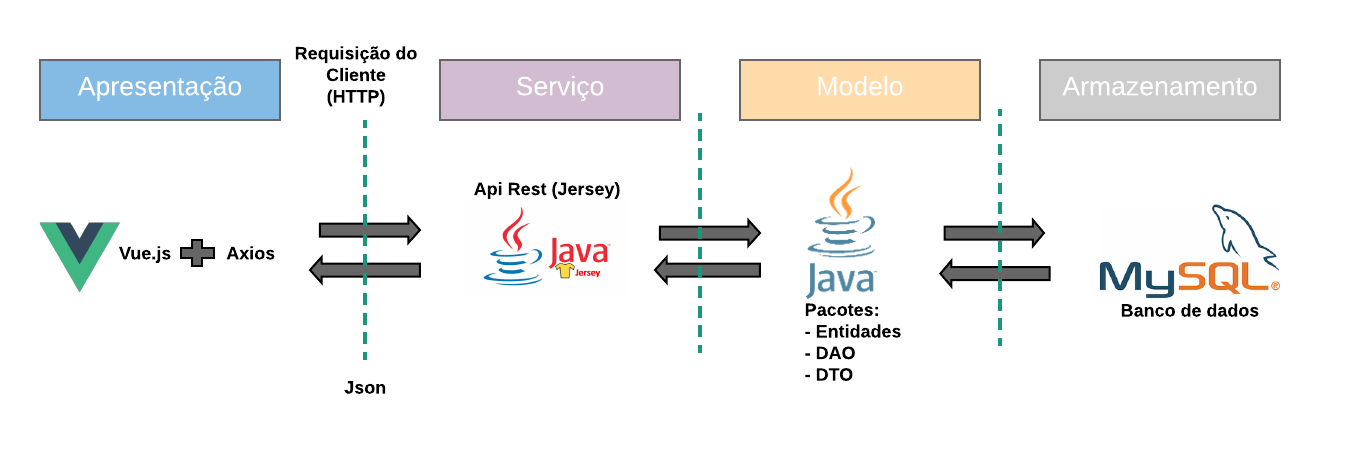
\includegraphics[keepaspectratio=true,scale=0.2]{figuras/arquitetura.png}
	\caption{Arquitetura geral do sistema}
	\label{fig2}
\end{figure}

\subsection{Ferramentas}

Para o desenvolvimento de uma solucão de software, deve-se considerar diversos
fatores, como: afinidade com as tecnologias de auxílio ao desenvolvimento, recursos disponibilizados pela tecnologia 
(frameworks, bibliotecas e etc), documentação da tecnologia entre outros fatores que podem influenciar diretamente
na construção do sistema.

No desenvolvimento desta ferramenta, a mesma foi dividida em duas áreas principais: backend e frontend. Para cada uma destas
áreas, apresentamos a seguir as ferramentas utilizadas.


O Desenvolvimento (Miolo ou Corpo do Trabalho) é subdividido em seções de 
acordo com o planejamento do autor. As seções primárias são aquelas que 
resultam da primeira divisão do texto do documento, geralmente 
correspondendo a divisão em capítulos. Seções secundárias, terciárias, 
etc., são aquelas que resultam da divisão do texto de uma seção primária, 
secundária, terciária, etc., respectivamente.

As seções primárias são numeradas consecutivamente, seguindo a série 
natural de números inteiros, a partir de 1, pela ordem de sua sucessão no 
documento.

O Desenvolvimento é a seção mais importante do trabalho, por isso exigi-se 
organização, objetividade e clareza. É conveniente dividi-lo em pelo menos 
três partes:

\begin{itemize}

	\item Referencial teórico, que corresponde a uma análise dos trabalhos 
	relevantes, encontrados na pesquisa bibliográfica sobre o assunto. 
	\item Metodologia, que é a descrição de todos os passos metodológicos 
	utilizados no trabalho. Sugere-se que se enfatize especialmente em (1) 
	População ou Sujeitos da pesquisa, (2) Materiais e equipamentos 
	utilizados e (3) Procedimentos de coleta de dados.
	\item Resultados, Discussão dos resultados e Conclusões, que é onde se 
	apresenta os dados encontrados a análise feita pelo autor à luz do 
	Referencial teórico e as Conclusões.

\end{itemize}

\section{Uso de editores de texto}

O uso de programas de edição eletrônica de textos é de livre escolha do autor. 

